\documentclass[a4paper,12pt]{article}
\usepackage{graphicx}
\usepackage[left=30mm, right=30mm, top=30mm, bottom=35mm]{geometry}
\usepackage{amsmath}
\usepackage{siunitx}
\usepackage{booktabs}
\usepackage{fancyhdr}
\usepackage{url}
\pagestyle{fancy}
%-------------------------------------------------------------------------------
\lhead{\textbf{Spring 2020}}
\rhead{\textbf{CE394M Advanced Analysis in Geotechnical Engineering}}
\cfoot{\thepage}
%-------------------------------------------------------------------------------

\begin{document}
\begin{centering}
	\textbf{
		Assignment 00: Limit analysis\\
		Assigned: 22nd January 2020\\
		Due: 27th January 2020\\
	}
\end{centering}

\vspace{1em}
 
Perform short-term limit equilibrium analyses (upper and lower bound solutions) of the slope shown below using the Optum G2 software. Compute the factor of safety and plot the magnitude of displacement from the limit analyses. 

This assignment has step-by-step instructions on performing limit analyses using Optum G2.

\begin{figure}[!h]
	\centering
	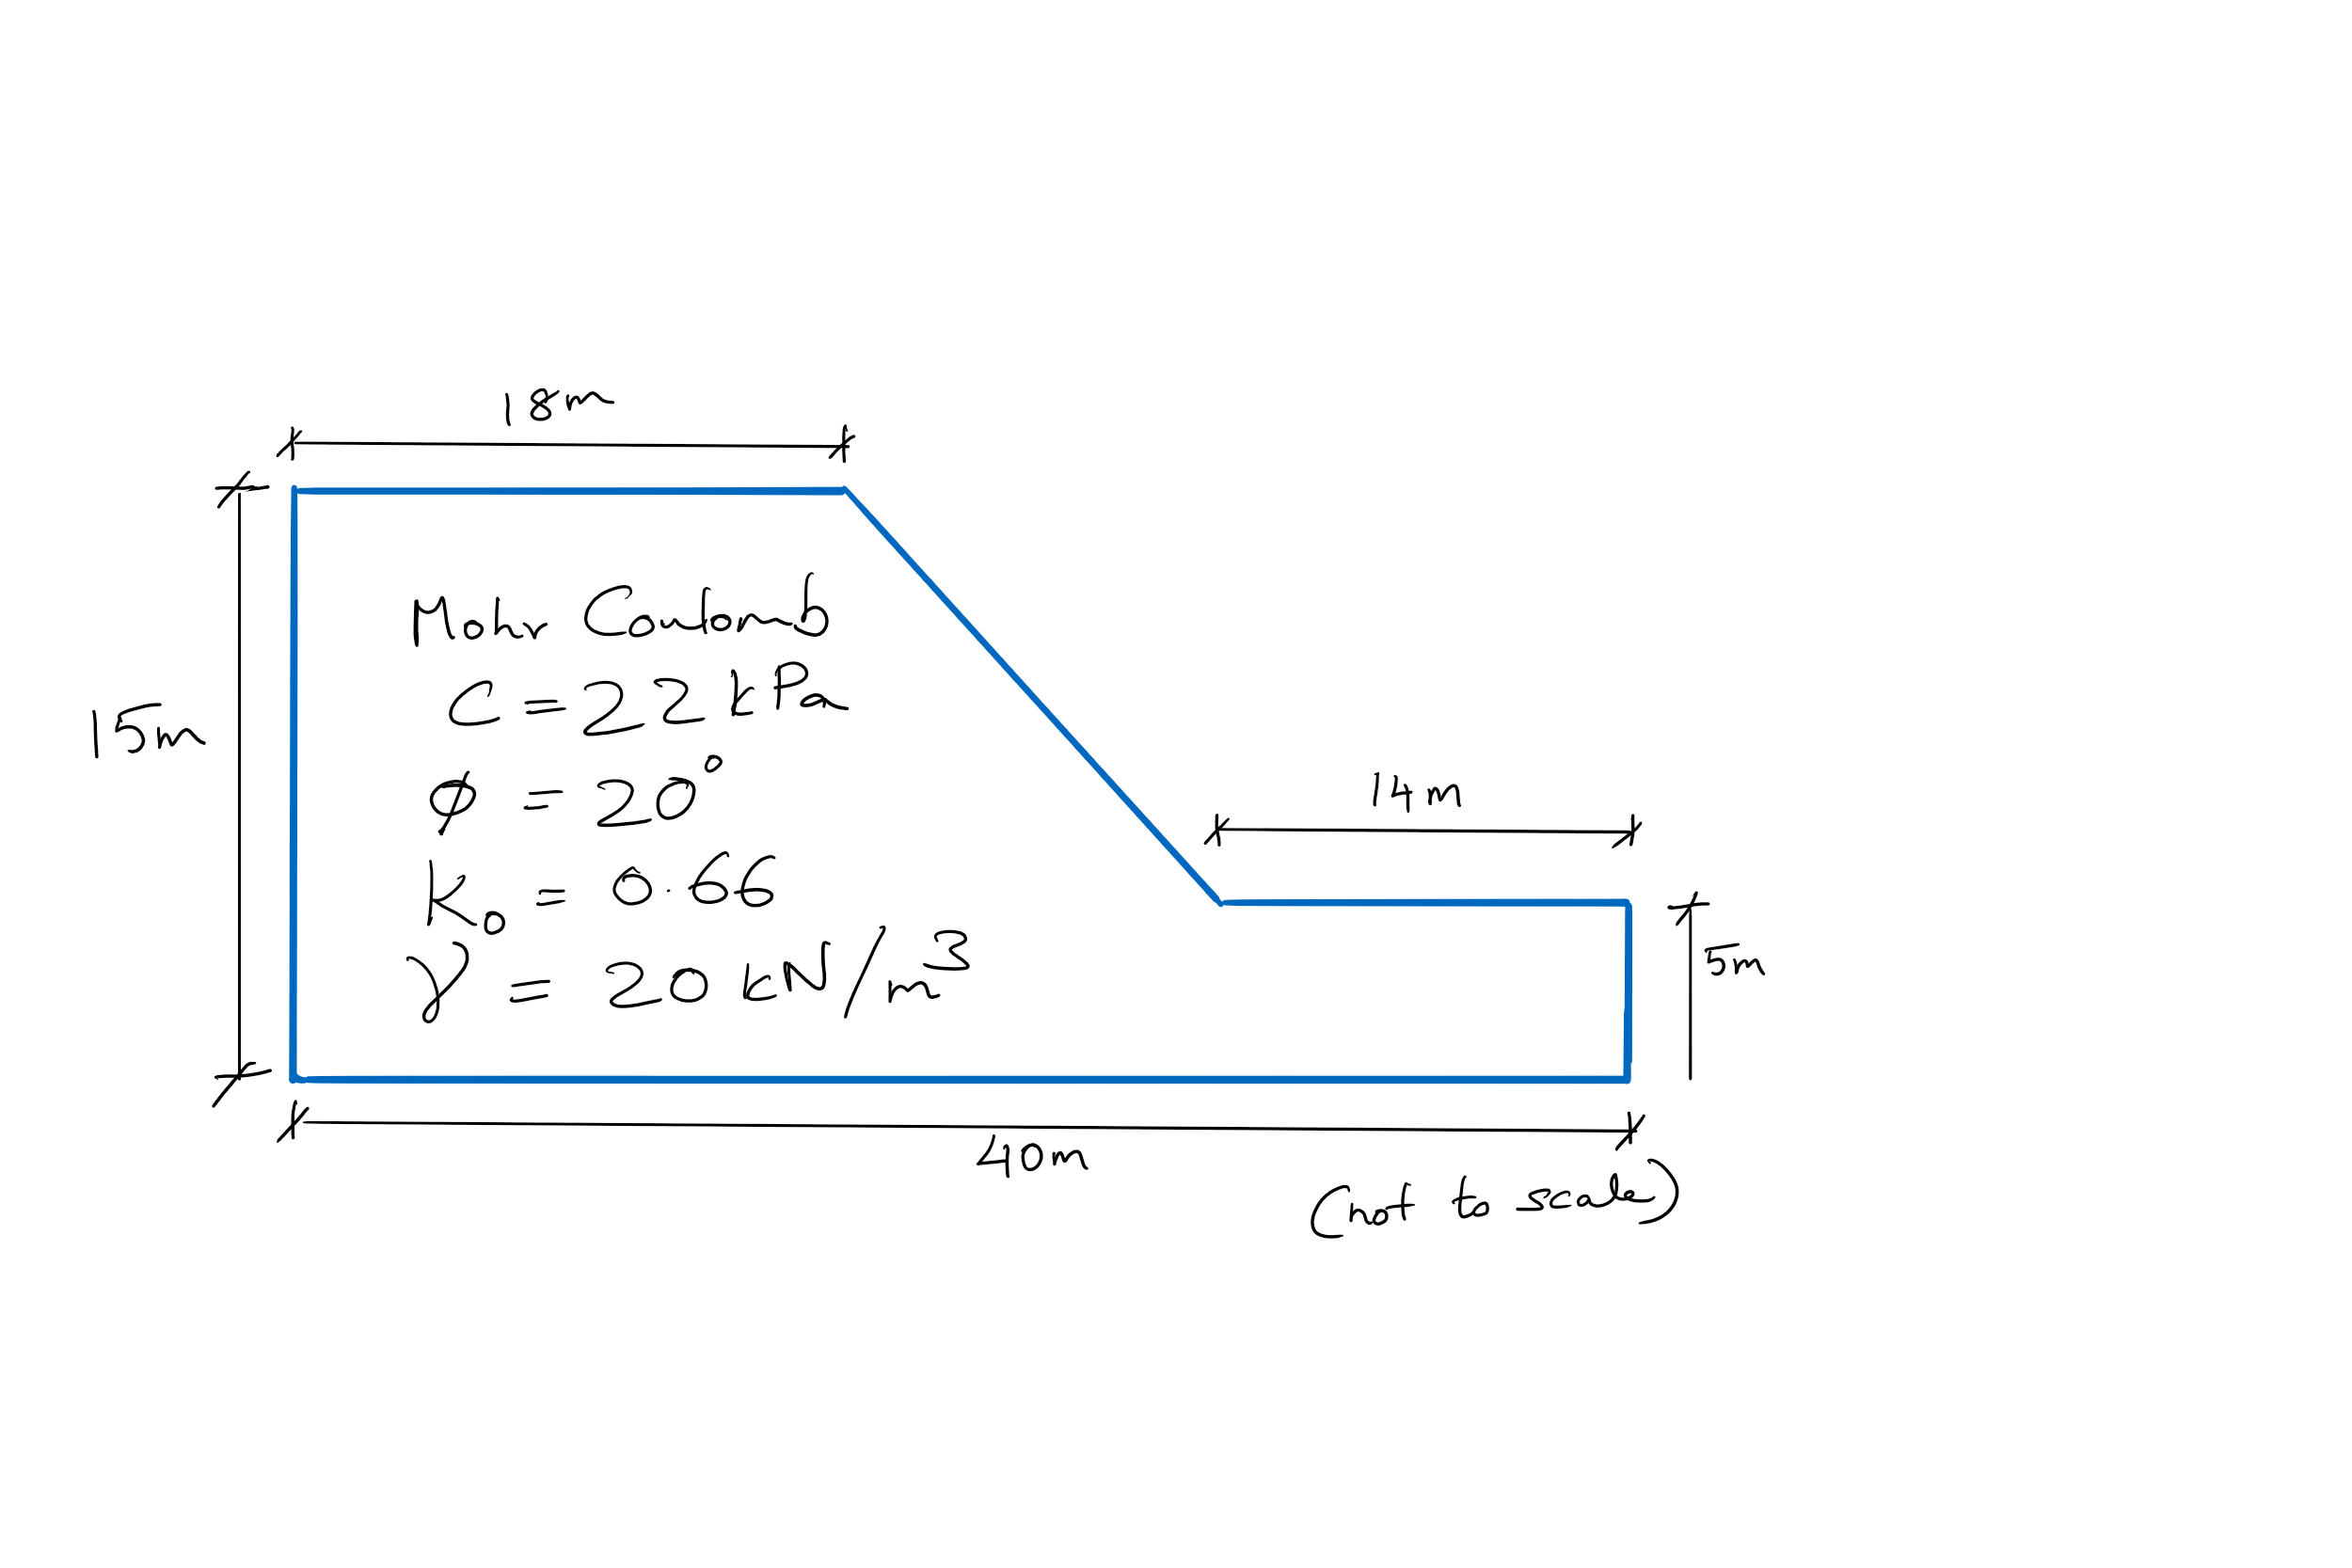
\includegraphics[width=0.75\textwidth]{figs/slope.png}
\end{figure}

\begin{enumerate}
	\item A free academic version of Optum G2 can be obtained by registering at: ~\url{https://optumce.com/academic/academic-license/optumg2-register-new-user/}
	
	\item After installation using the student license, open a new project. For your convenience the geometry of the slope is provided to you as a CAD drawing (DXF file) in Canvas. Import the DXF to the Current Stage as shown below.
	
	\begin{figure}[!h]
		\centering
		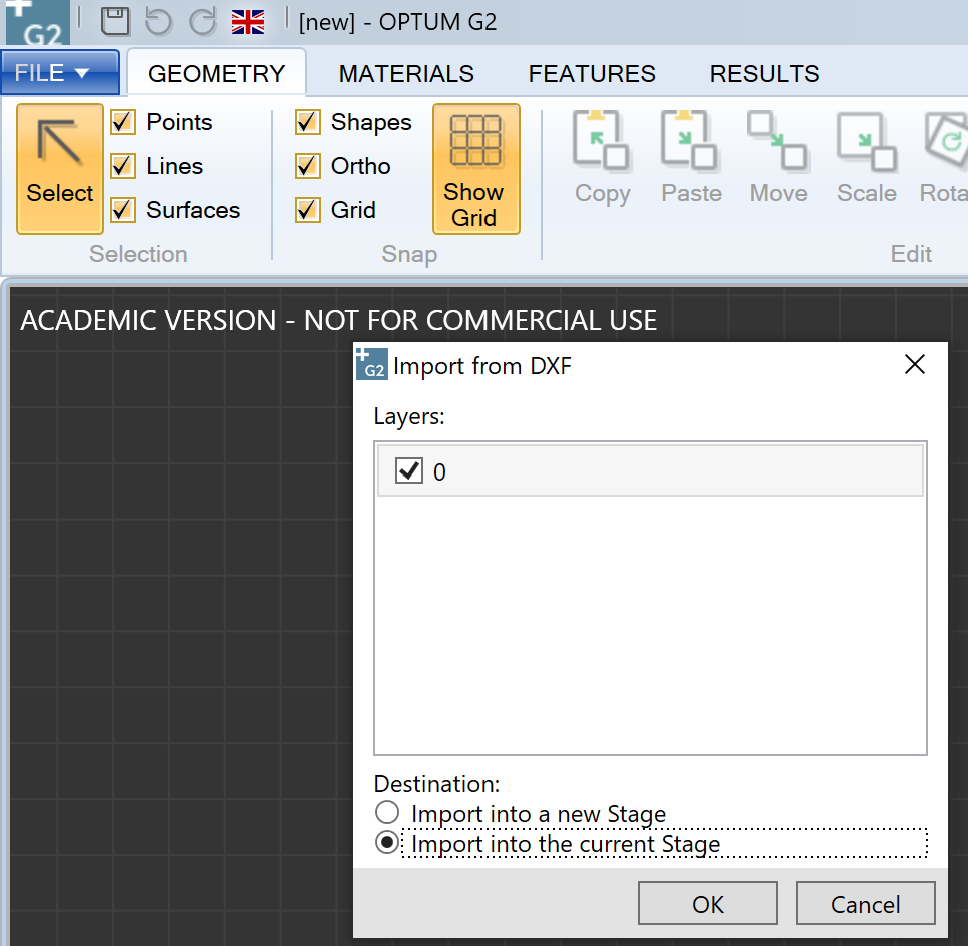
\includegraphics[width=0.75\textwidth]{figs/import-dxf.png}
		\caption{Import DXF}
	\end{figure}
	
	\item Select the geometry, this should highlight the slope and then choose the `MATERIALS' tab from the top ribbon. Select the Mohr Coulomb material model (MC Basic). Specify the strength parameters, unit weight and K0 for the initial condition (which might be under Not relevant to analysis section). The material parameters are shown below. Set both dry and saturated unit weights to be the same.

	\begin{table}[!h]
		\centering
		\begin{tabular}{ll}
			\toprule
			\textbf{Properties}     & \textbf{Values} \\
			\midrule
			cohesion (c) & 22 kPa    \\
			friction ($\phi$)   & $20^o$   \\
			unit weight ($\gamma$)   & 20 $kN/m^3$    \\
			K0             & 0.66  \\
			\bottomrule
		\end{tabular}
	\end{table}
	
	\begin{figure}[!h]
		\centering
		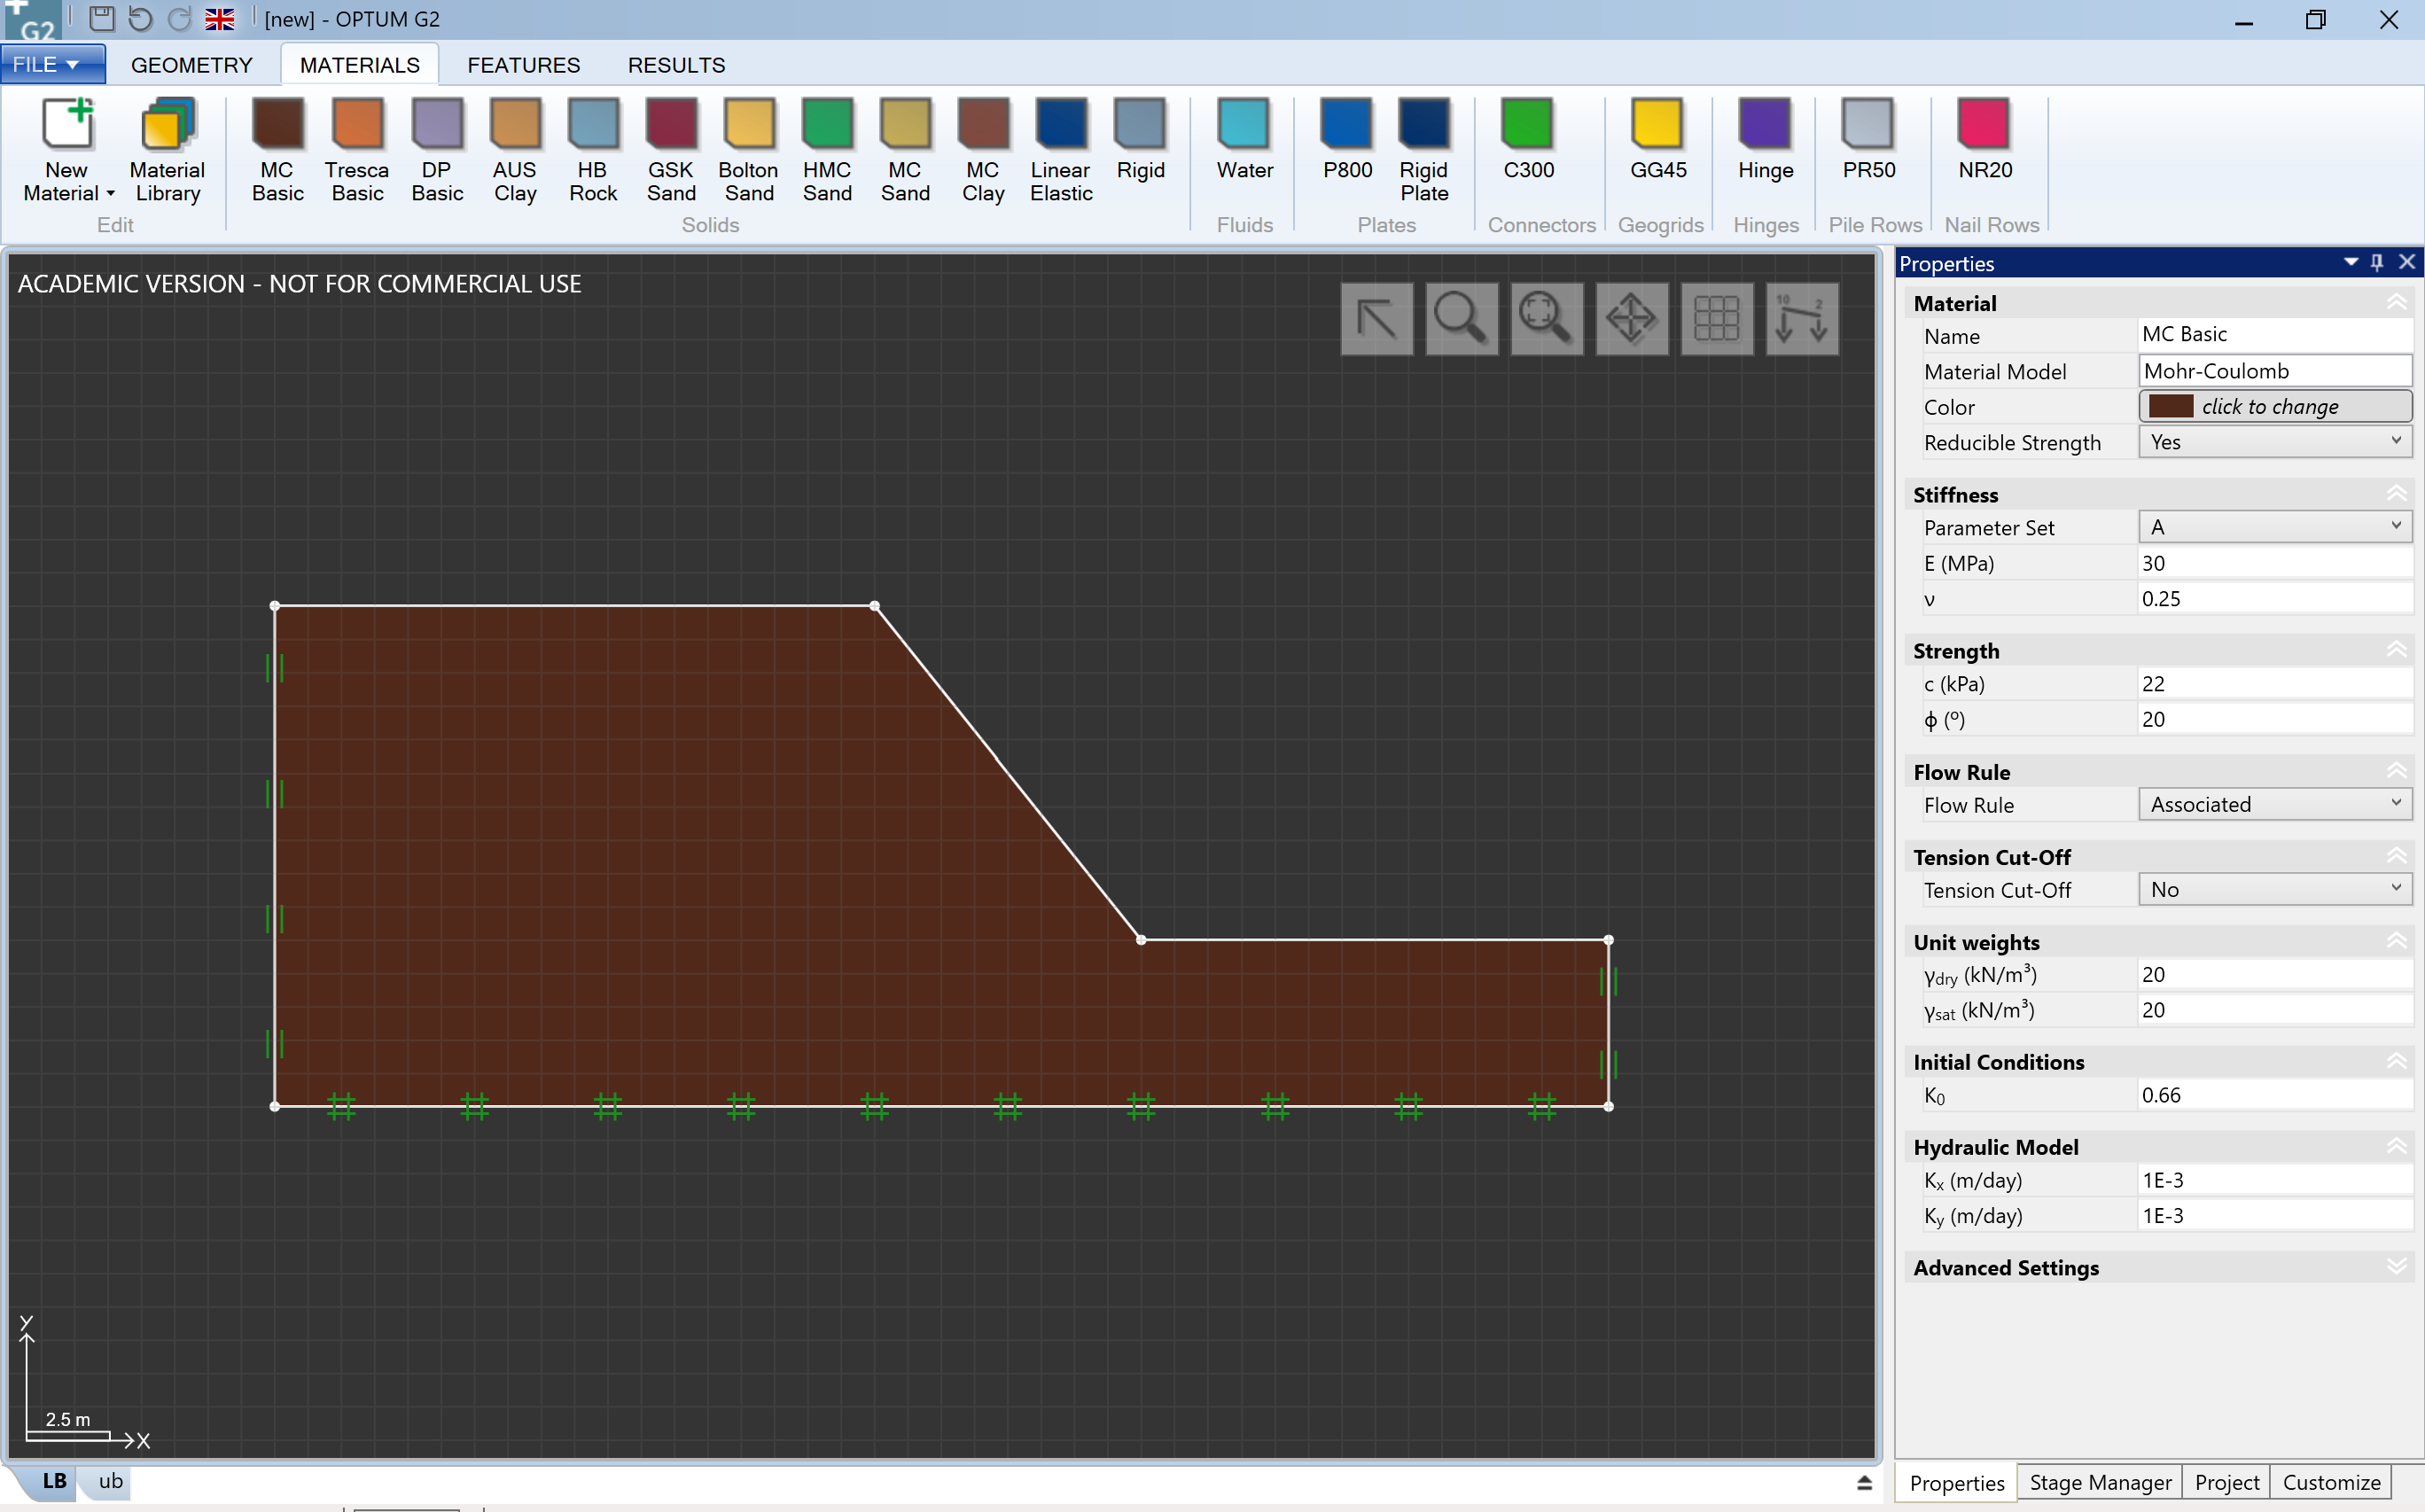
\includegraphics[width=0.75\textwidth]{figs/apply-material.png}
		\caption{Apply material}
	\end{figure}

	\item The next step is to apply boundary conditions. This is done by selecting ``Standard Fixities" in the ``Features" tab. Roller boundaries will be applied on the sides allowing vertical displacements, but restraining horizontal movements. The bottom boundary is completely fixed.
	
	\begin{figure}[!h]
		\centering
		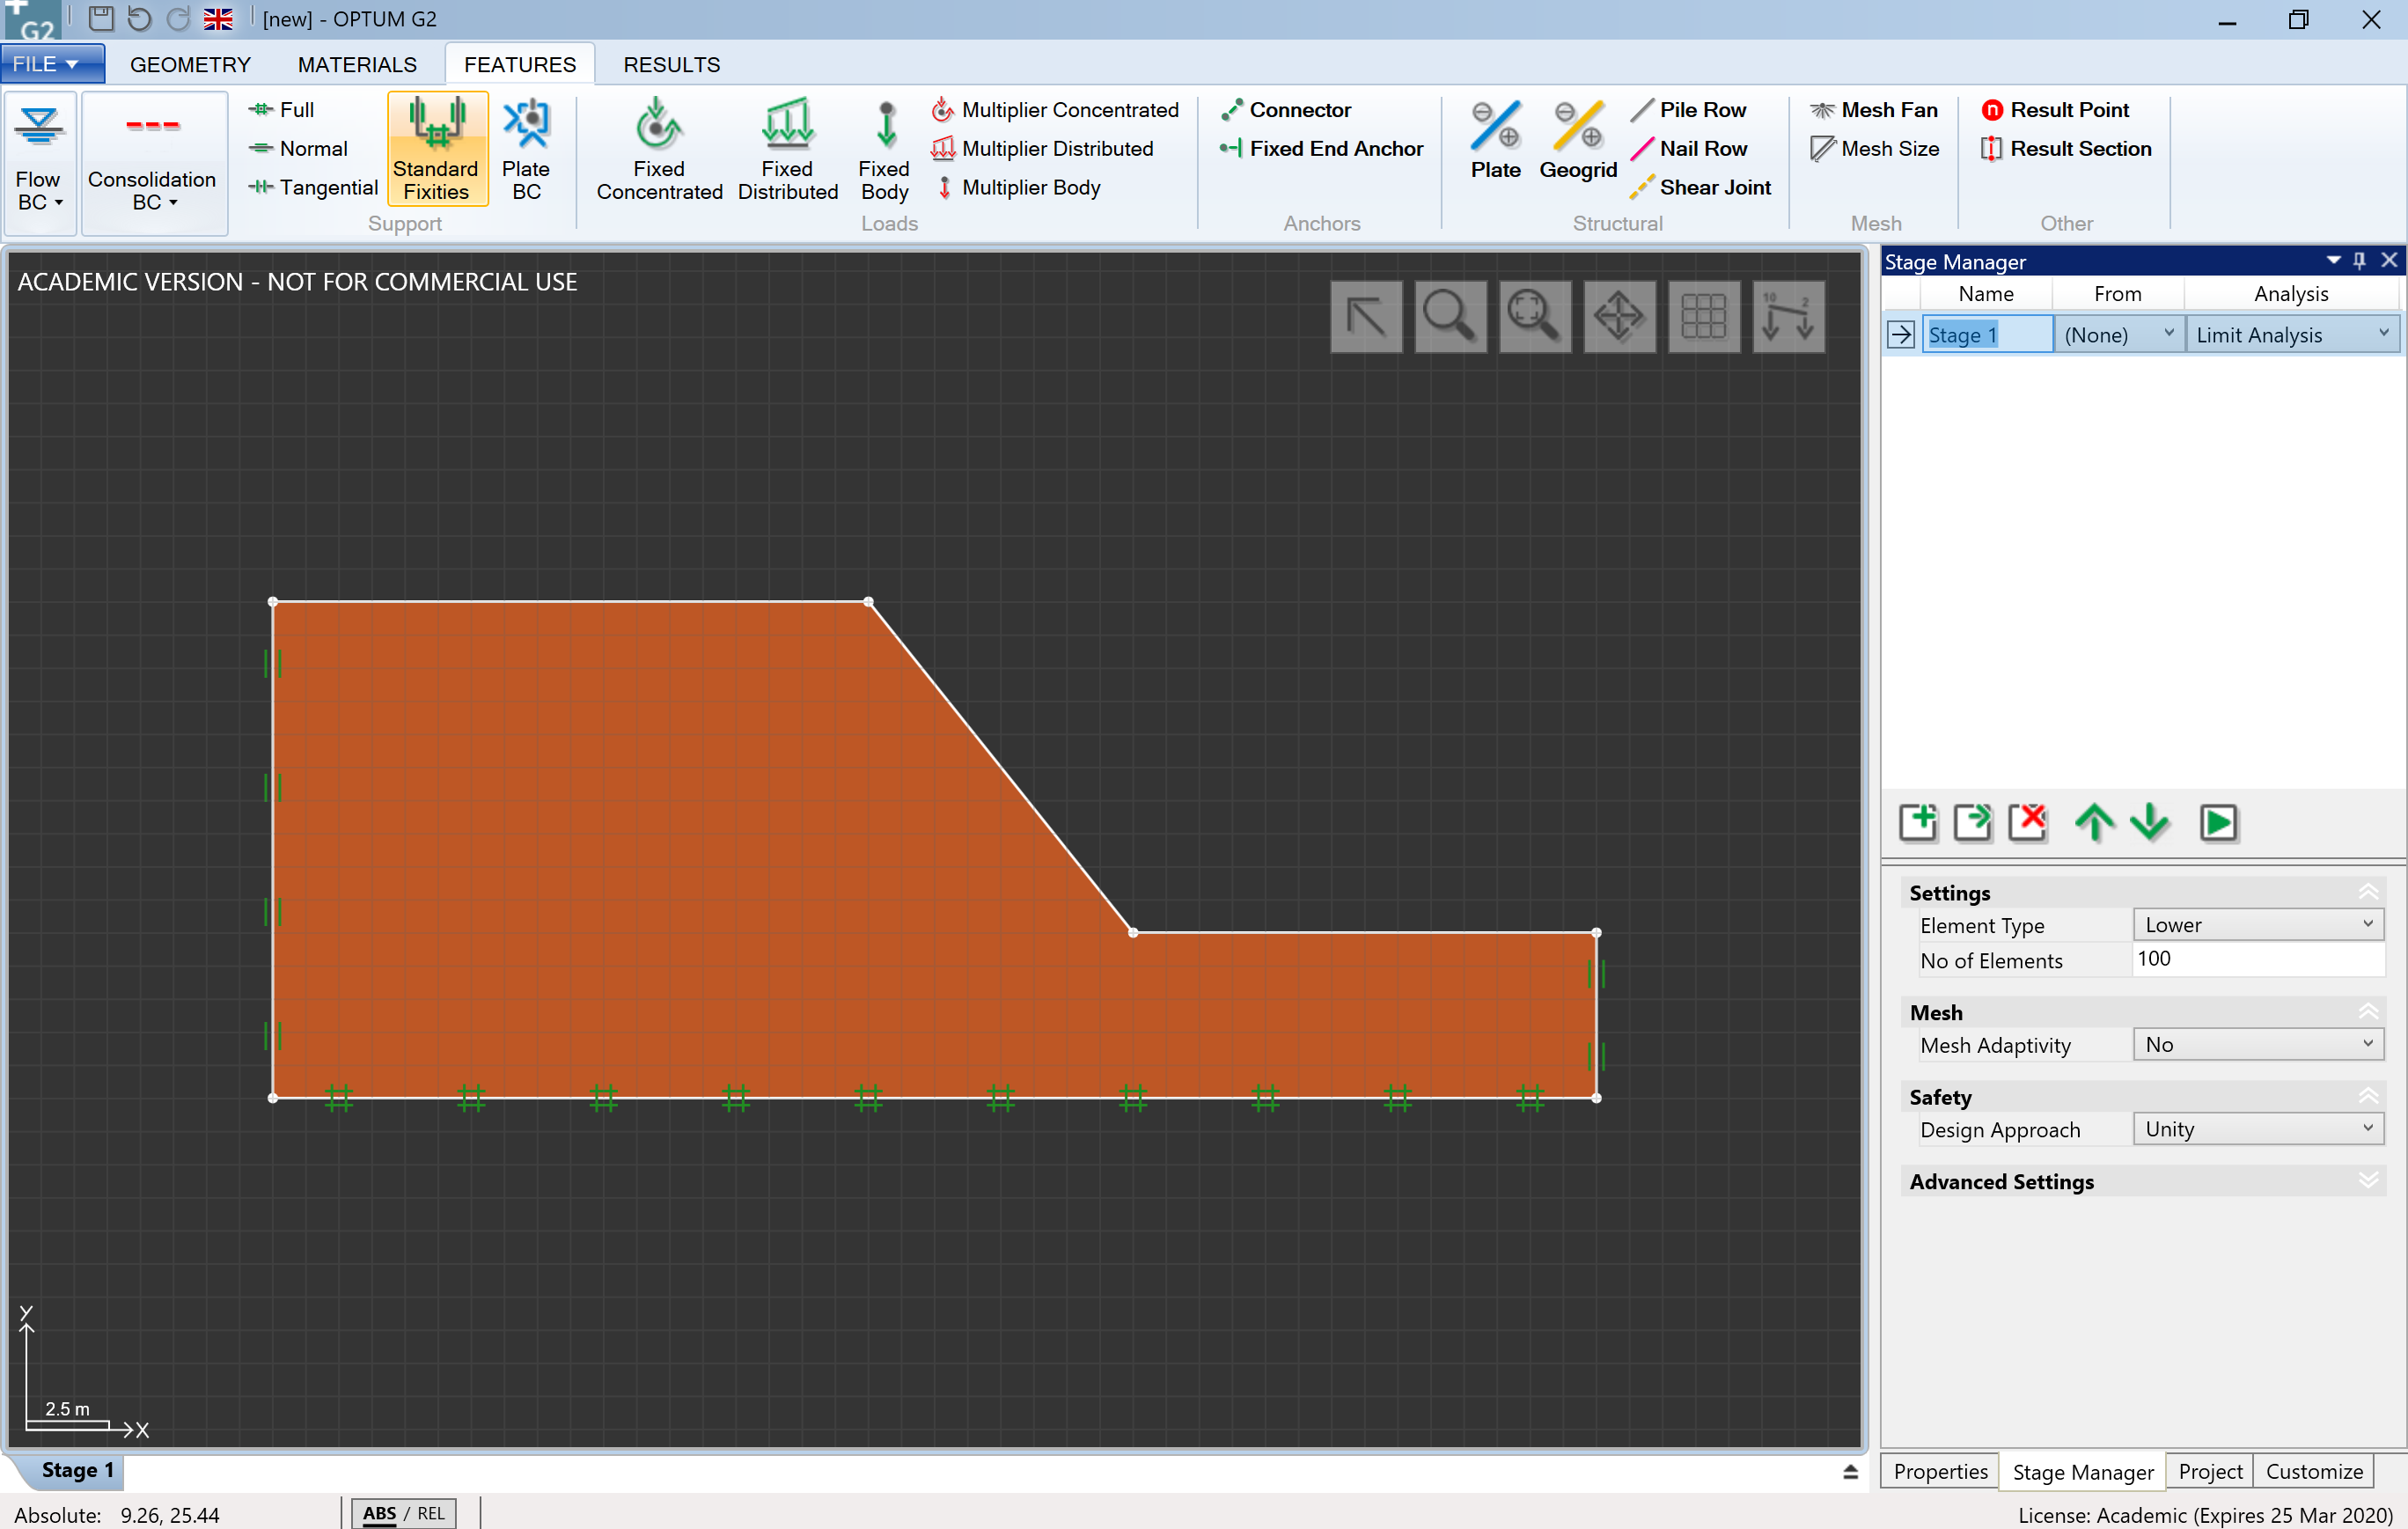
\includegraphics[width=0.75\textwidth]{figs/fixities.png}
		\caption{Apply boundary conditions}
	\end{figure}

	\item We are now ready to perform the analysis. Choose the ``Stage manager" tab on the right bottom from the panel on the right. To perform a lower bound analysis, choose the Analysis type as ``Limit Analysis" and the Element type in settings as ``Lower". Ensure that a minimum of 100 elements are used in the analysis with adaptive meshing enabled. Under advanced settings, specify the multiplier as `Gravity' this will increase the gravity in stages, until the slope fails. The analysis will be carried out to analyze the short-term stability of the slope. 

	\begin{figure}[!h]
		\centering
		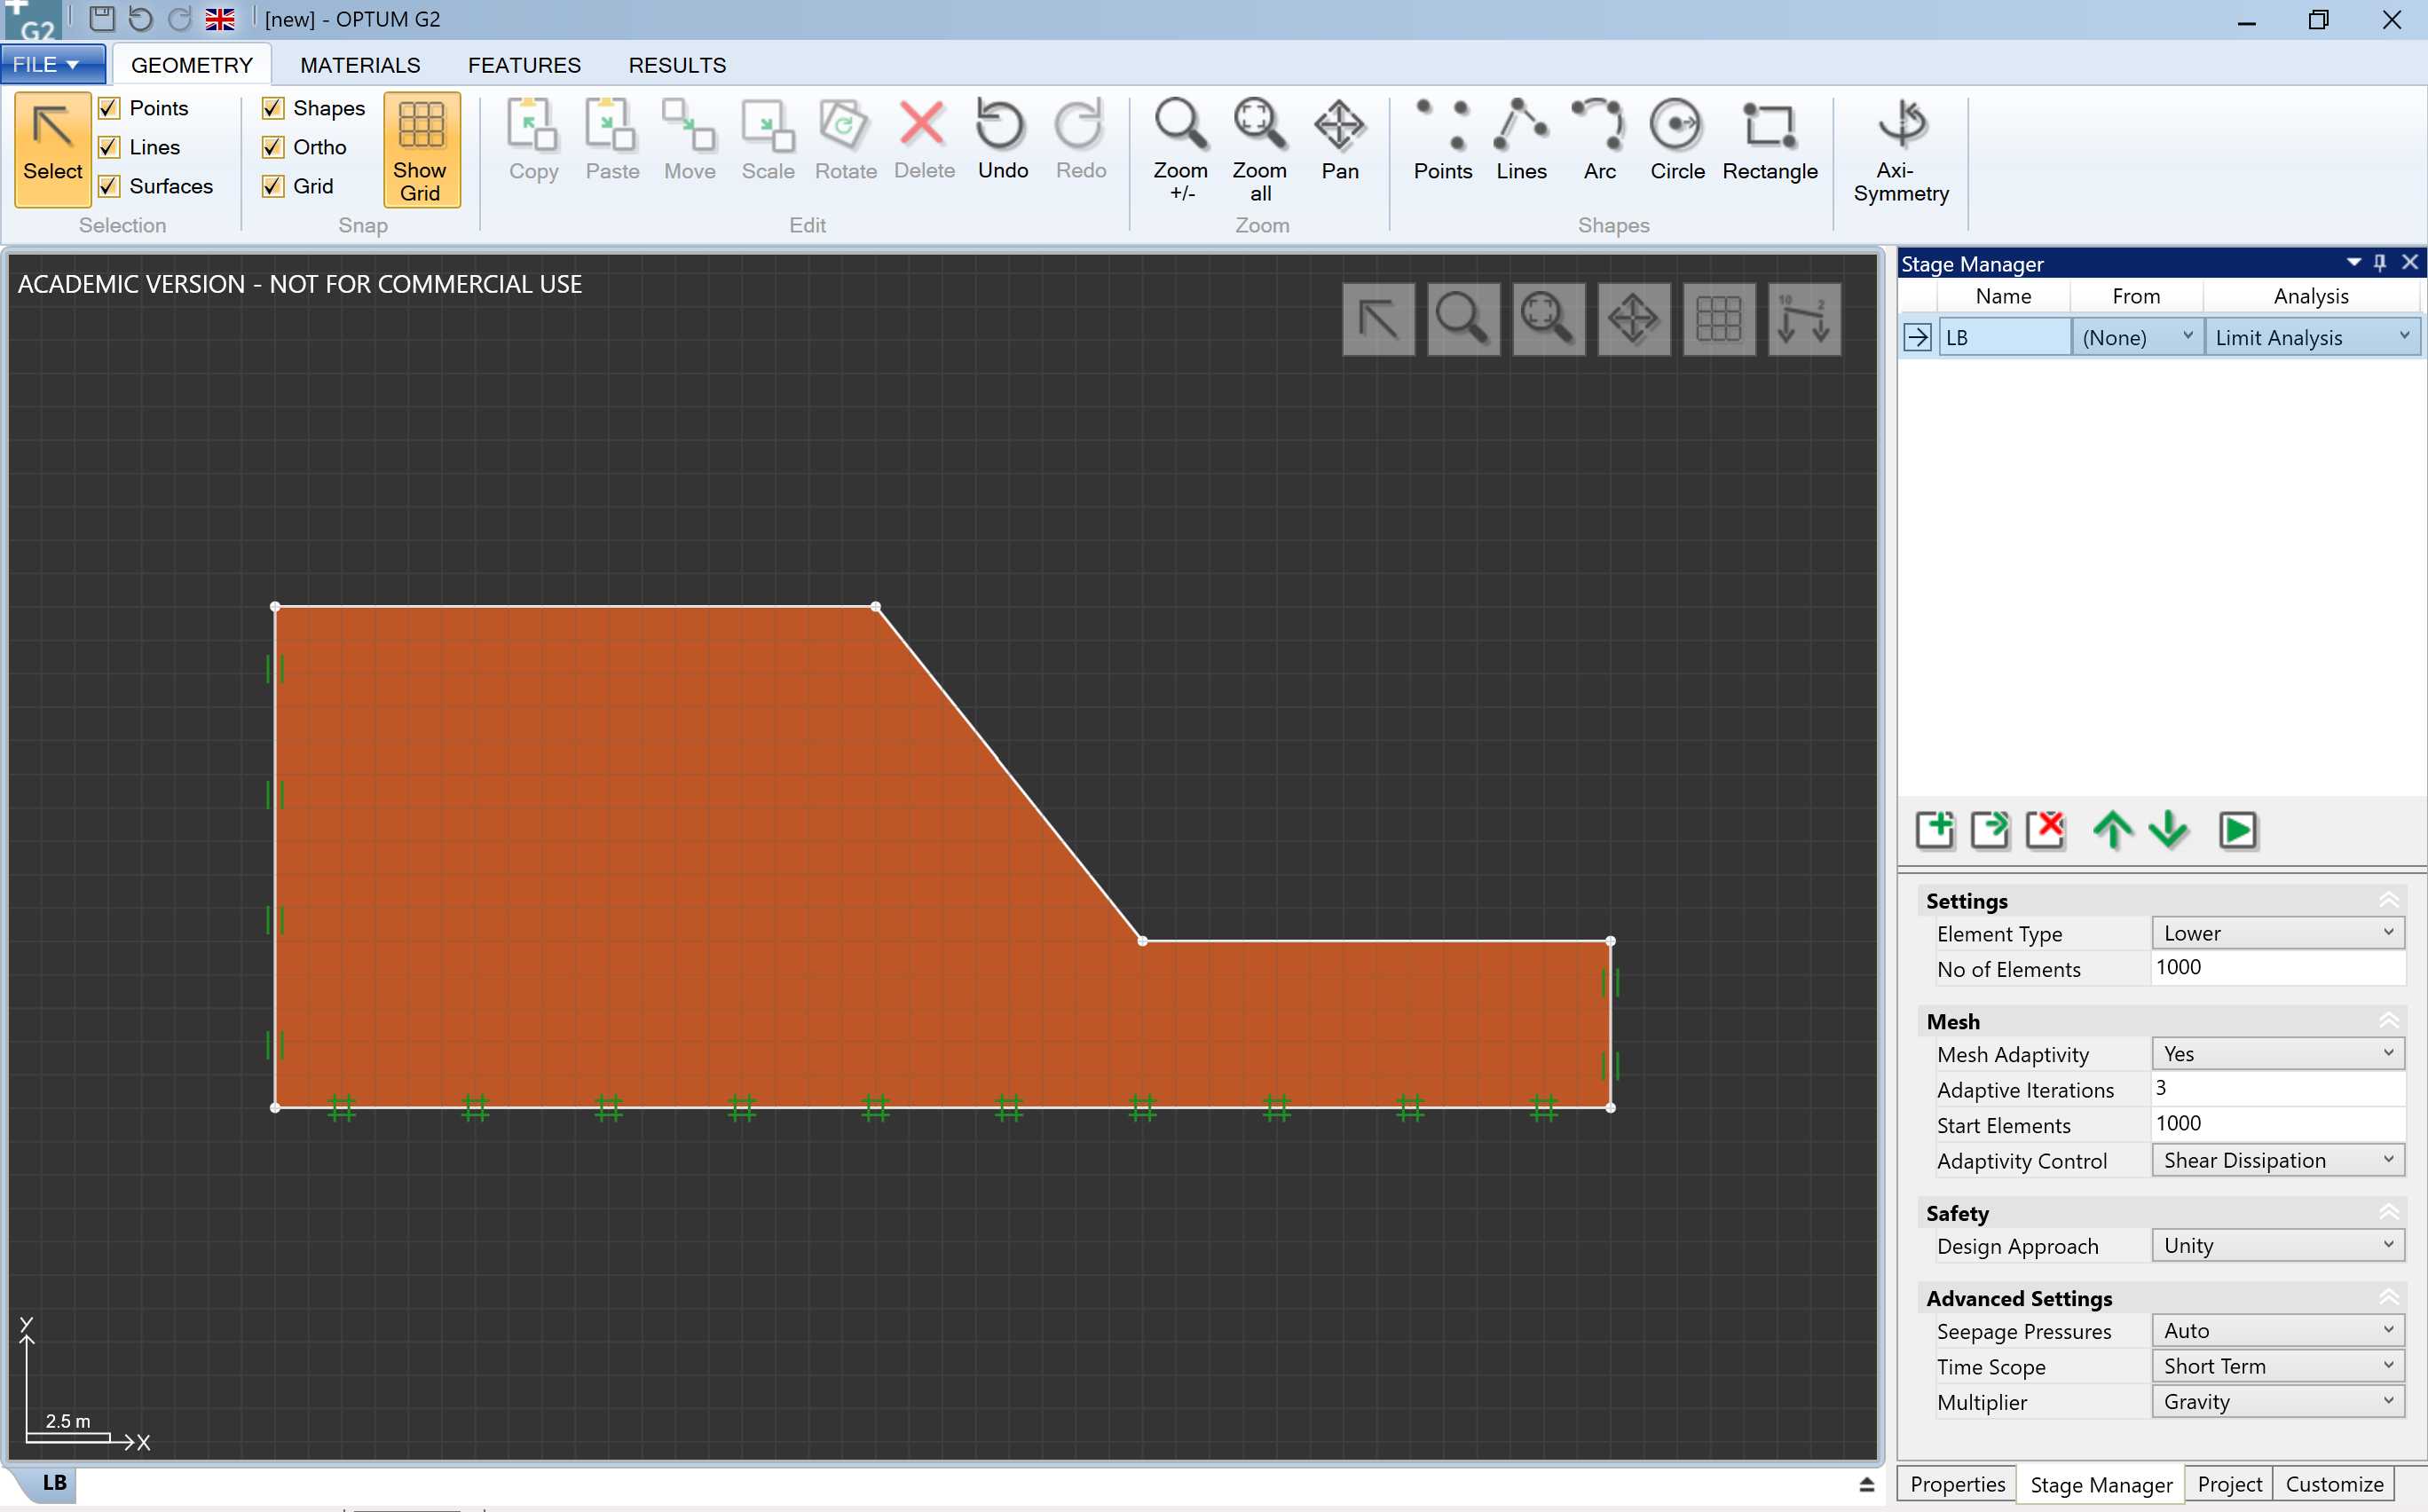
\includegraphics[width=0.75\textwidth]{figs/lb.png}
		\caption{Lower bound analysis}
	\end{figure}	

	\item To perform the upper bound analysis, clone the stage 1, which should be renamed as `LB'. Then change the element type in the new stage `UB' as ``Upper". When ready choose ``Run analysis" button. 
	
	\item The software will perform both the lower and upper bound analyses and present the factor of safety against failure. Comment on the factor of safety obtained from both the analyses. Plot the magnitude of displacement from both the analyses. 
	
	
	\begin{figure}[!h]
		\centering
		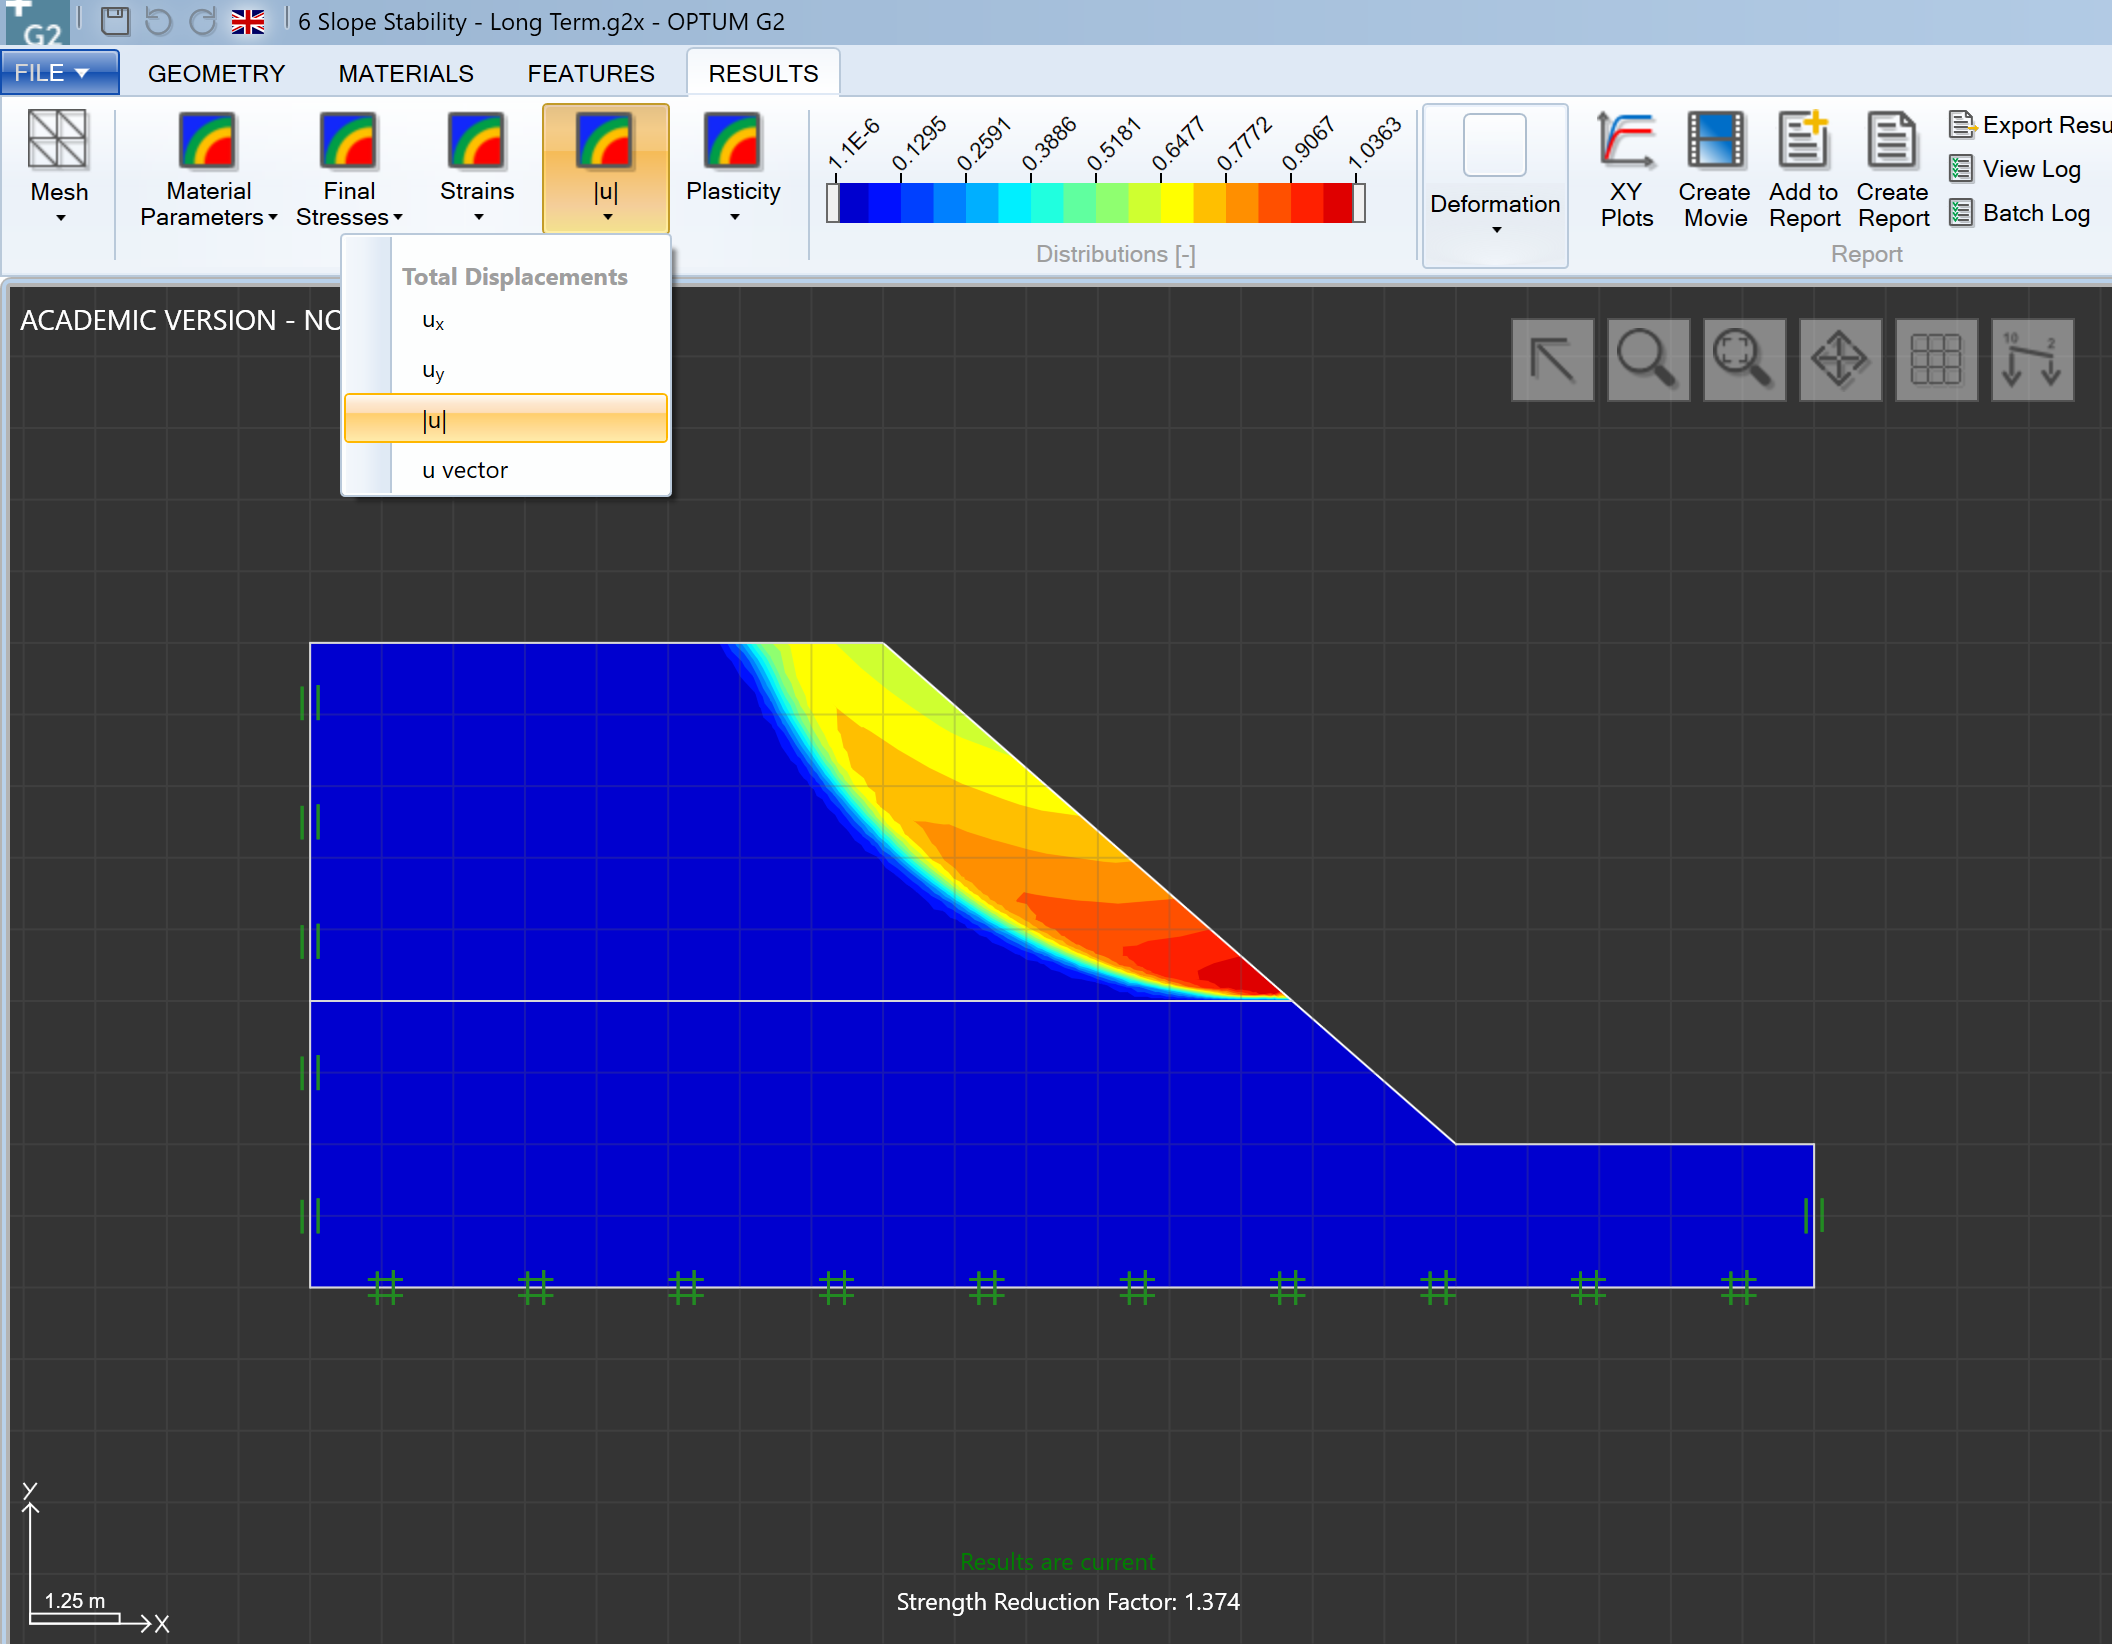
\includegraphics[width=0.75\textwidth]{figs/results.png}
		\caption{Magnitude of displacement (not the solution for this assignment).}
	\end{figure}	
\end{enumerate}

\end{document}

